\section{Materiais e métodos}

Para este trabalho primeiramente foi realizada um revisão de literatura simples
para conhecer mais sobre o assunto tratado, observando pesquisas com problemas semelhantes e 
as soluções obtidas. 

Como metodologia principal foi utilizada uma pesquisa-ação tendo como objeto de estudo um projeto de uma organização descrita no capítulo \ref{pesquisa_acao}. A pesquisa-ação realizada foi composta das fases representadas na Figura \ref{fig:metodologia}.

	
\begin{figure}[!htb]
\centering
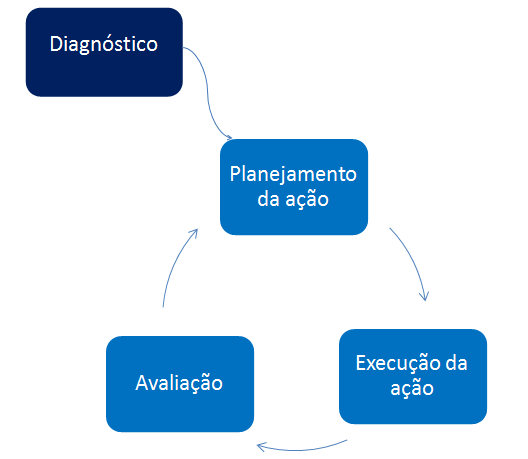
\includegraphics[scale=1]{figuras/pesquisaacao.png}
\caption{Fases da pesquisa-ação. Baseado em \cite{artigo_pesquisa_acao}}
\label{fig:metodologia}
\end{figure}

\pagebreak

De acordo com \citeonline{artigo_pesquisa_acao}, uma pesquisa-ação é composta das seguintes fases: 
	\begin{itemize}
		\item \textbf{Diagnóstico:} Essa fase tem como objetivo principal conhecer a situação atual e o problema relacionado ao objeto de estudo. Para realização do diagnóstico foram aplicados questionários. 
		\item \textbf{Planejamento da ação:} Essa fase tem como objetivo propor uma ação para resolver o problema diagnosticado, definindo o número de ciclos, as atividades da ação, os envolvidos e como a ação será avaliada.
		\item \textbf{Execução da ação:} Essa fase consiste em executar a ação proposta e acompanhá-la.
		\item \textbf{Avaliação da ação:} Essa fase consiste na avaliação da ação executa a fim de realizar melhorias no próximo ciclo para a ação proposta.
	\end{itemize}

